\documentclass[12pt]{article}
\usepackage[utf8]{inputenc}
\usepackage[spanish]{babel}
\usepackage{graphicx}
\usepackage{float}
\usepackage{hyperref}
\usepackage{amsmath}
\usepackage{amssymb}
\usepackage[
    type={CC},
    modifier={by-nc-sa}, 
    version={3.0},
]{doclicense}
\usepackage{verbatim}

\title{Memoria Métodos de clasificación}
\author{Nerea Jiménez González\\ Yhondri Acosta Novas}
\date{Abril 2020}

\begin{document}

\maketitle
\begin{figure}[H]
    \centering
    
\includegraphics[width=1\textwidth]{3-2016-07-21-Marca UCM Monocromo Negro.png}
\end{figure}

\newpage
\tableofcontents
\listoffigures
\newpage

\section{Detalles de la implementación}
\subsection{Lenguaje utilizado}
Para la implementación, se utiliza el lenguaje JAVA.
\subsection{Procedimiento seguido para la implementación}
Para la primera implementación hemos elegido el algoritmo borroso.\\
Este algoritmo recibe los datos de las clases y los datos de los centros iniciales. \\
El algoritmo ejecuta una función \textit{performIteration} que devuelve un booleano que indica si es necesario seguir iterando según el parámetro épsilon que nos da la práctica.\\
Lo primero que hace el método \textit{performIteration} es calcular la distancias. Para ello iteramos sobre la matrix \textit{dataMatrix} que contiene los datos de las 2 clases. Dentro del bucle llamamos al método \textit{calculateDistancesBetween} y que calcula \textit{dxx} siguiendo la fórmula $d_{ij}=\left \| x_{j}-v_{j} \right \|^{2}$.  El valor obtenido lo almacenamos en una matrix denominada \textit{distances}.\\
A continuación calculamos los grados de pertenencia. Para ello en un bucle iteramos sobre la matrix \textit{dataMatrix} que contiene los datos de las 2 clases. Este bucle llama al método \textit{calculateMembershipgrade}. Este método aplica la ecuación $P(v_{i}/x_{j})=\frac{1/d_{ij}^{1/(b-1)}}{\sum_{r=1}^{c}1/d_{rj}^{^{1/(b-1)}}}$. El resultado obtenido lo almacenamos en la matrix \textit{membershipGradesMatrix}. A continuación recalculamos los centros en un siguiente bucle y lo almacenamos en la variable \textit{initialCentroMatrix}.\\
Finalmente iteramos sobre los centros, obtenemos su distancia, y comparamos con épsilon. Si la distancia es mayor o igual que épsilon, hemos terminado las iteraciones, en caso contrario el método devolverá false indicado que necesita iterar de nuevo para hallar la solución.\\
Para obtener el resultado de un caso de prueba, utilizamos el método \textit{getClassForValues}. Este método itera sobre los valores y aplica el algoritmo Borroso con los datos anteriormente calculados. Por último construye un string con los datos obtenidos de la ejecución del algoritmo.

\subsection{Ampliaciones realizadas}
Para la ampliación hemos realizado tanto el algoritmo de Bayes como el de Lloyd.
\subsubsection{Algoritmo de Bayes}
Este algoritmo no necesita ningún parámetro extra, por lo que sólo recibe los datos de las muestras agrupadas por clases.\\
Lo primero que calculamos son las medias de cada clase mediante la función \textit{calculateAverage}. Para calcular las medias sumamos todas las matrices de muestras de cada clase con la función \textit{plusArray}, y despúes dividimos el resultado entre las cantidad de muestras de dicha clase con la función \textit{divide}. Estas dos funciones pertenece a la clase \textit{Matrix}. Hacemos esta operación para cada clase, y guardamos los resultados en las variables \textit{averageClassX}, donde x es el número de la clase a la que corresponda la media calculada.\\
Una vez tenemos ambas medias, ya podemos saber a qué clase pertenece una muestra dada. Para ello utilizamos la clase \textit{whichClassBelongTo}, que recibe una matriz con los datos de la muestra a clasificar.\\
En esta clase primero restamos a la muestra el centro de la clase que queremos comprobar si pertenece a esta con la función \textit{minus}, y después calculamos la distancia con la función \textit{distanceBayes}. La distancia más pequeña será la que decida a que clase pertenece nuestra muestra.

\subsubsection{Algoritmo de Lloyd}
Este algoritmo recibe los parámetros de tolerancia, número máximo de iteraciones y los centros a usar. La razón de aprendizaje no es un parámetro como tal ya que es una constante global. También reciben los datos de las muestras.\\
Lo primero que hacemos es actualizar los centros, para ello usamos la función \textit{updateCenters}. Esta función realiza las iteraciones necesarias actualizando el centro que se vaya eligiendo. La condición de parada para dejar de iterar es o bien que llegue hasta el máximo de iteraciones, \textit{maxIterations}, o bien que ya no sea necesario seguir actualizando. Para esta segunda condición usamos la función \textit{keepUpdating}, la cuál calcula la distancia Euclidea y si es menor que la toleracia calculandola con ambos centros, devuelve true, de forma que se para de iterar. En caso contrario, devuelve false y se sigue iterando si no ha llegado a\textit{ maxIterations} iteraciones.\\
Cada iteración recorre todas las muestras de ambas clases. Para cada muestra se decide que centro actualizar, para lo cual utilizamos la función \textit{whichCenterToUpdate}. Esta función recibe la muestra en forma de array la cual va a decidir que centro vamos a actualizar. Para ello se realizal los cálculos necesarios para obtener la distancia con ambos centros. La distancia más pequeña decide que centro actualizar.\\
Una vez sabemos que centro vamos a actualizar, utilizamos la función \textit{updateCenterChoosed}, a la cuál pasamos el centro que hemos elegido y la muestra que hemos utilizado para ello. Esta función actualiza el centro mediante la función 
$c_{j}(k+1)=c_{j}(k)+\gamma(k)[x(k)-c_{j}(k)]$.\\
Los centros actualizados se van guardado en la matriz \textit{updateCenters}, mientras que la matriz \textit{oldCenters} contiene los valores de los centros antes de comenzar la iteración. Esto lo hacemos porque necesitamos saber ambos valores para la función \textit{keepUpdating}. La matriz \textit{updateCenters} pasa a ser oldCenters al comienzo de una nueva iteración.\\
Una vez tenemos los centros actualizados, ya podemos saber a que clase pertenece una muestra dada. Para ello utilizamos la función \textit{whichClassBelongTo}, la cual recibe una matriz con los datos de la muestra a clasificar. Para saber a que clase pertenece, calculamos las distancias respecto a cada centro, y aquella con valor más pequeño es a la que pertenece la clase.

\section{Código ejecutable}
Se adjunta en el archivo formato zip, con nombre\textbf{ Código}.
\subsection{Simulación}
Para las simulaciones vamos a usar el ejemplo \textbf{TestIris03.txt}.
\subsubsection{Algoritmo Bayes}
\begin{figure}[H]
    \centering
    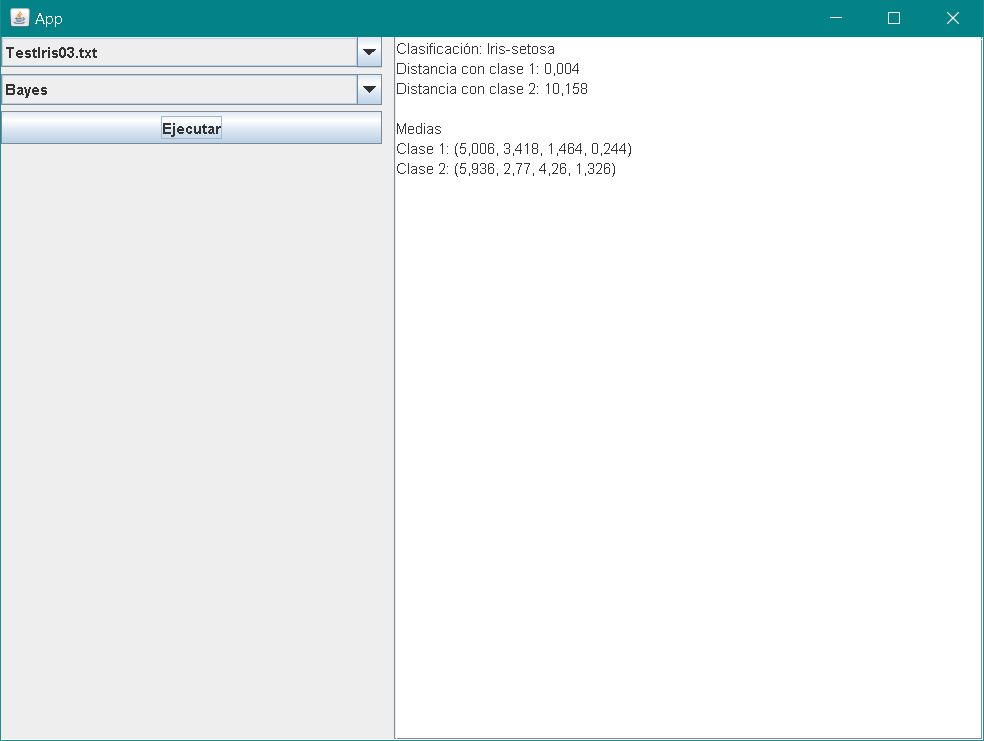
\includegraphics[width=1\textwidth]{bayes.JPG}
    \caption{Ejemplo de Bayes}
\end{figure}
\subsubsection{Algoritmo Borroso}
\begin{figure}[H]
    \centering
    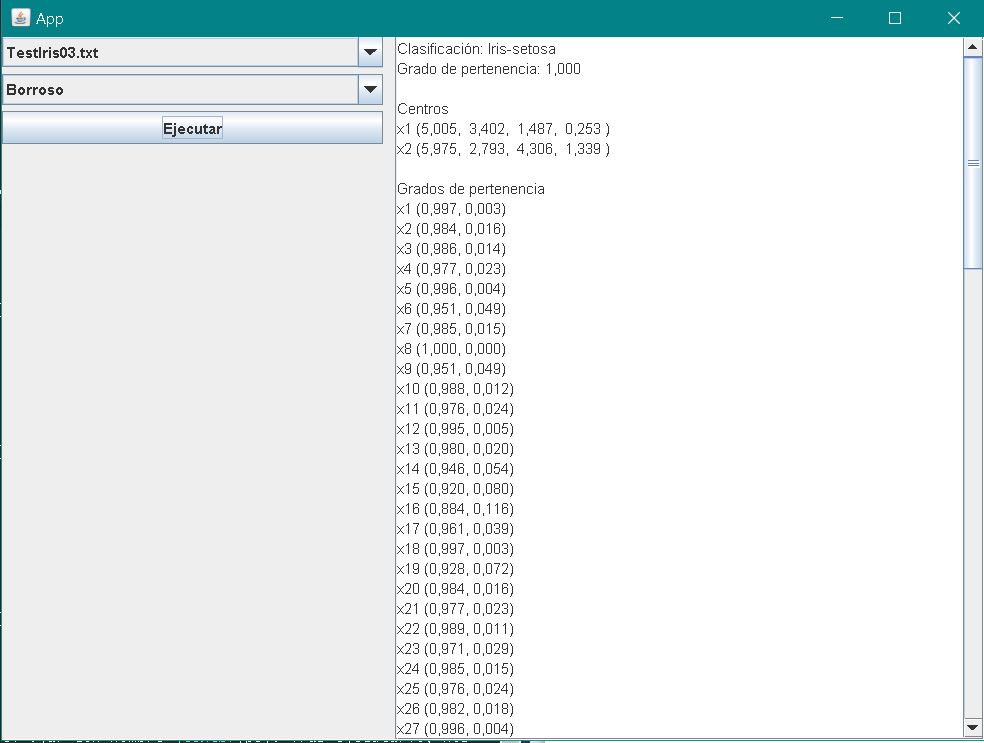
\includegraphics[width=1\textwidth]{borroso.JPG}
    \caption{Ejemplo de Borroso}
\end{figure}

\subsubsection{Algoritmo de Lloyd}
\begin{figure}[H]
    \centering
    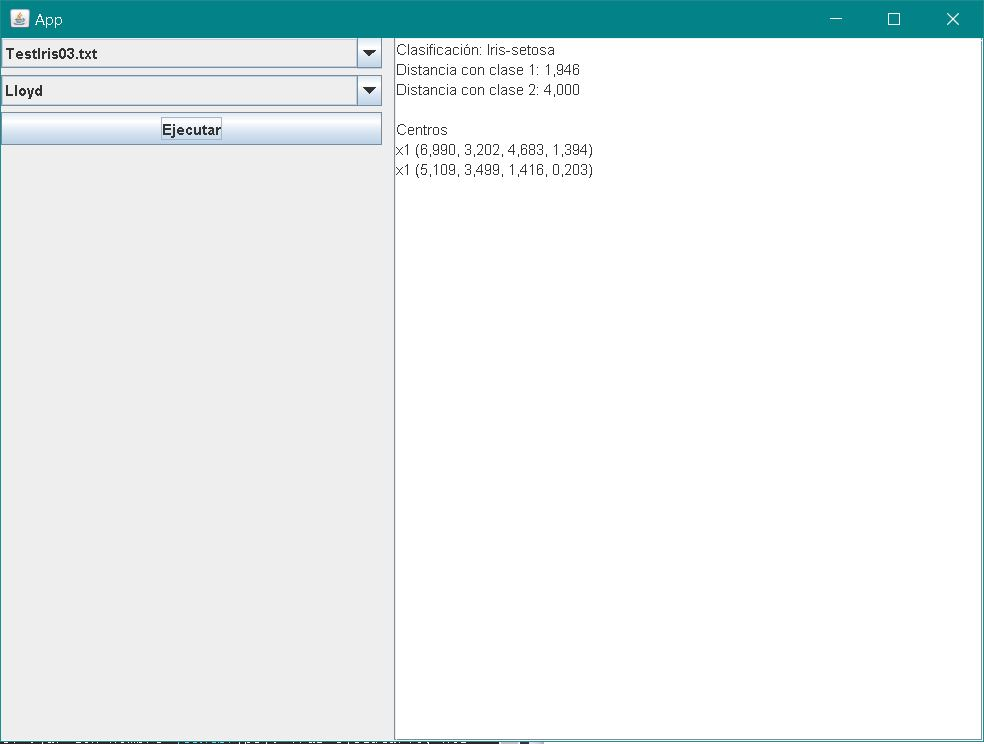
\includegraphics[width=1\textwidth]{lloyd.JPG}
    \caption{Ejemplo de Lloyd}
\end{figure}

\section{Manual de usuario}
Hacer doble click en el .jar con nombre \textbf{p3}. Tras ejecutarlo, nos aparecerá la siguiente ventana:
\begin{figure}[H]
    \centering
    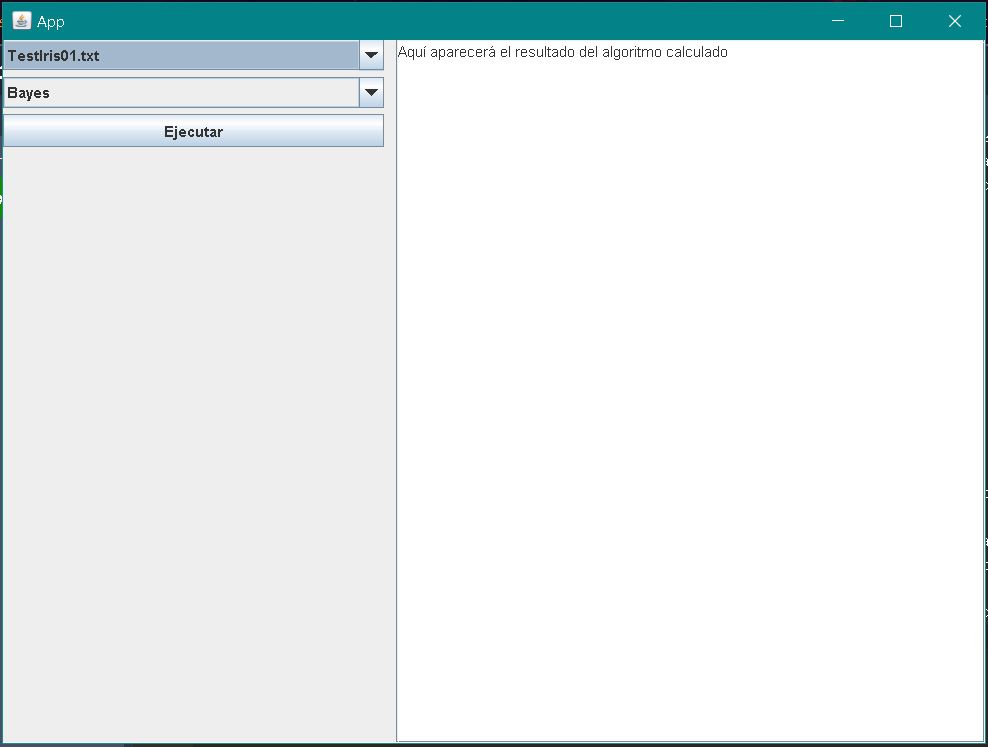
\includegraphics[width=1\textwidth]{primera.JPG}
    \caption{Ventana inicial}
\end{figure}
En la primera barra de selección, elegimos el ejemplo de los tres dados que queremos clasificar. En la segunda barra elegimos con qué algoritmo queremos clasificarlo. Una vez elegido, clickeamos \textbf{Ejecutar.}
\begin{figure}[H]
    \centering
    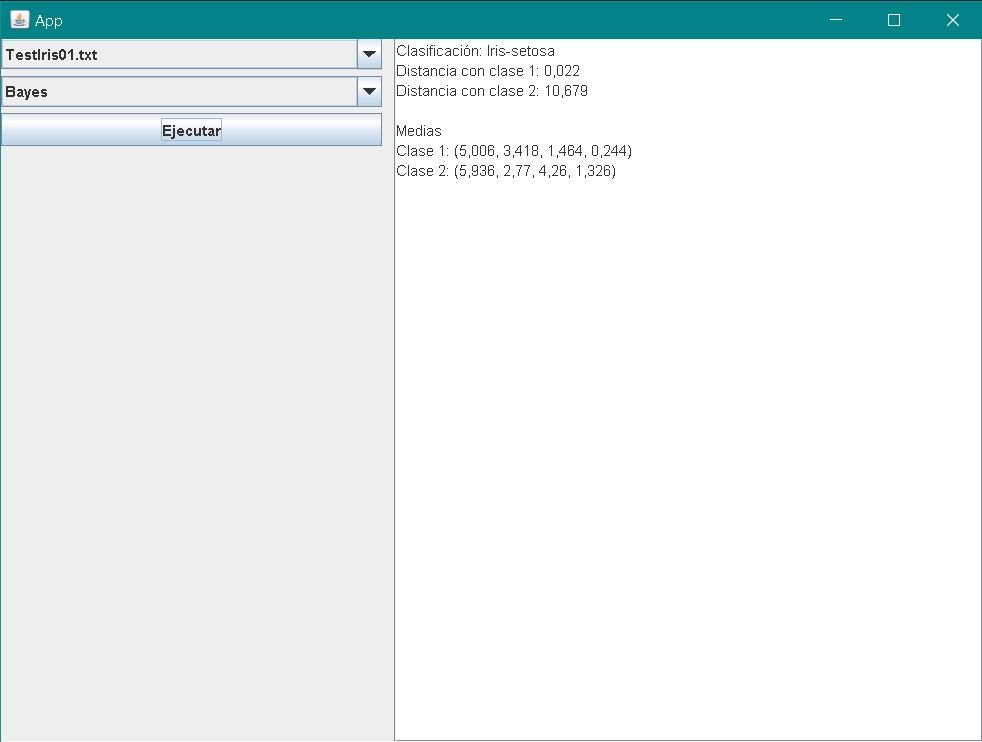
\includegraphics[width=1\textwidth]{segunda.JPG}
    \caption{Resultados tras ejecutar algoritmo}
\end{figure}
En la parte derecha de la ventana, nos aparecerán los datos de la clasificación realizada. Depende del algoritmo, se muestran unos datos u otros.
\newpage
\vspace*{\fill}
\begin{verbatim}
    Memoria Práctica 3
    Mayo 2020
    Ult. actualización 29 de abril de 2020
\end{verbatim}
\LaTeX{} lic. LPPL \& Nerea Jiménez y Yhondri Acosta \& CC-ZERO
\doclicenseThis
\end{document}
